
\section{Experimento BRDF Ashikhmin-Shirley Alternativa}


Nesse caso, foi realizada uma versão alternativa do experimento descrito na \autoref{sec:ashikhmin-shirley}. As equações apresentadas na \autoref{fig-ashikhmin-shirley-alternative-eqlang-latex} foram simplificadas, e algumas delas foram combinadas em uma única expressão. Além disso, nesta versão, foram utilizadas constantes diferentes, como cor difusa e fatores de multiplicação, entre outros. O código-fonte em \texttt{EquationLang} está disponível no \autoref{cod-ashikhmin-shirley-alternative-eqlang}. Os códigos gerados em GLSL estão no \autoref{cod-ashikhmin-shirley-alternative-glsl-pt-1} e no \autoref{cod-ashikhmin-shirley-alternative-glsl-pt-2}. A renderização dos objetos 3D pode ser observada na \autoref{fig-ashikhmin-shirley-alternative-eqlang}, e os \textit{plots} correspondentes estão na \autoref{fig-ashikhmin-shirley-alternative-plots}.
%%%%%%%%%%%%%%%%%%%%%%%%%%%%%%%%%%%%%%%%%%%%%%%%%
\subsection{Representação em documento \LaTeX{}}
%%%%%%%%%%%%%%%%%%%%%%%%%%%%%%%%%%%%%%%%%%%%%%%%%
\begin{figure}[H]
  \caption{\label{fig-ashikhmin-shirley-alternative-eqlang-latex}
  \small Equações da BRDF do experimento Ashikhmin-Shirley$_2$ (alternativa) em documento \LaTeX{}.}
    \begin{center}
        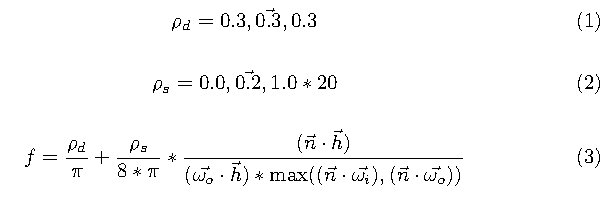
\includegraphics[scale=0.92]{./Imagens/brdfs/ashikhmin-shirley-alternative.pdf}
    \end{center}
\end{figure}

%%%%%%%%%%%%%%%%%%%%%%%%%%%%%%%%%%%%%%%%%%%%%%%%%
\subsection{Código GLSL Gerado}
%%%%%%%%%%%%%%%%%%%%%%%%%%%%%%%%%%%%%%%%%%%%%%%%%
\begin{codigo}[H]
    \caption{\small Saída do compilador: código GLSL da BRDF deste experimento (parte 1 de 2).}
    \label{cod-ashikhmin-shirley-alternative-glsl-pt-1}
\begin{lstlisting}[language=C, inputencoding=utf8]
analytic ::begin parameters
#[type][name][min val][max val][default val]
::end parameters
::begin shader
//////////// START OF BUILTINS DECLARTION ////////////
vec3 var_0_vec_h;
vec3 var_3_vec_n;
float var_10_theta_h;
float var_11_theta_d;
float var_1_pi;
float var_2_epsilon;
vec3 var_4_vec_omega_i;
float var_5_theta_i;
float var_6_phi_i;
vec3 var_7_vec_omega_o;
float var_8_theta_o;
float var_9_phi_o;
//////////// END OF BUILTINS DECLARTION ////////////

//////////// START OF USER DECLARED ////////////
vec3 var_12_rho_d;
vec3 var_13_rho_s;
vec3 var_14_f;
//////////// END OF USER DECLARED ////////////
\end{lstlisting}
\end{codigo}

\begin{codigo}[H]
    \caption{\small Saída do compilador: código GLSL da BRDF deste experimento (parte 2 de 2).}
    \label{cod-ashikhmin-shirley-alternative-glsl-pt-2}
\begin{lstlisting}[language=C, inputencoding=utf8]
//////////// START FUNCTIONS DECLARATIONS ////////////
//////////// END FUNCTIONS DECLARATIONS ////////////

vec3 BRDF(vec3 L, vec3 V, vec3 N, vec3 X, vec3 Y) {

  //////////// START OF BUILTINS INITIALIZATION ////////////
  var_0_vec_h = normalize(L + V);
  var_3_vec_n = normalize(N);
  var_1_pi = 3.141592653589793;
  var_2_epsilon = 1.192092896e-07;
  var_4_vec_omega_i = L;
  var_5_theta_i = atan(var_4_vec_omega_i.y, var_4_vec_omega_i.x);
  var_6_phi_i = atan(sqrt(var_4_vec_omega_i.y * var_4_vec_omega_i.y +
                          var_4_vec_omega_i.x * var_4_vec_omega_i.x),
                     var_4_vec_omega_i.z);
  var_7_vec_omega_o = V;
  var_8_theta_o = atan(var_7_vec_omega_o.y, var_7_vec_omega_o.x);
  var_9_phi_o = atan(sqrt(var_7_vec_omega_o.y * var_7_vec_omega_o.y +
                          var_7_vec_omega_o.x * var_7_vec_omega_o.x),
                     var_7_vec_omega_o.z);
  var_10_theta_h = acos(dot(var_0_vec_h, N));
  var_11_theta_d = acos(dot(var_0_vec_h, var_4_vec_omega_i));
  //////////// END OF BUILTINS INITIALIZATION ////////////

  var_12_rho_d = vec3(0.3, 0.3, 0.3);
  var_13_rho_s = (vec3(0.0, 0.2, 1.0) * 20.0);
  var_14_f = ((var_12_rho_d / var_1_pi) +
              ((var_13_rho_s / (8.0 * var_1_pi)) *
               ((dot(var_3_vec_n, var_0_vec_h)) /
                ((dot(var_7_vec_omega_o, var_0_vec_h)) *
                 max((dot(var_3_vec_n, var_4_vec_omega_i)),
                     (dot(var_3_vec_n, var_7_vec_omega_o)))))));

  return vec3(var_14_f);
}
\end{lstlisting}
\end{codigo}

%%%%%%%%%%%%%%%%%%%%%%%%%%%%%%%%%%%%%%%%%%%%%%%%%
\subsection{Código Fonte em \texttt{EquationLang}}
%%%%%%%%%%%%%%%%%%%%%%%%%%%%%%%%%%%%%%%%%%%%%%%%%
\begin{codigo}[H]
    \caption{\small Código-fonte da BRDF deste experimento.}
    \label{cod-ashikhmin-shirley-alternative-eqlang}
\begin{lstlisting}[language=tex, frame=none, inputencoding=utf8]

\begin{document}

\begin{equation}
    \rho_{d} = \vec{0.3,0.3,0.3}
\end{equation}

\begin{equation}
    \rho_{s} = \vec{0.0,0.2,1.0}*20
\end{equation}

\begin{equation}
f = \frac{\rho_{d}}{\pi} + \frac{\rho_{s}}{8*\pi} *
\frac{({\vec{n}}\cdot{\vec{h}})}
{({\vec{\omega_{o}}}\cdot{\vec{h}}) *
\max(({\vec{n}}\cdot{\vec{\omega_{i}}}),
({\vec{n}}\cdot{\vec{\omega_{o}}}))}
\end{equation}

\end{lstlisting}
\end{codigo}

%%%%%%%%%%%%%%%%%%%%%%%%%%%%%%%%%%%%%%%%%%%%%%%%%
\subsection{Visualização do Resultado}
%%%%%%%%%%%%%%%%%%%%%%%%%%%%%%%%%%%%%%%%%%%%%%%%%
\begin{figure}[H]
    \caption{\small{\textit{Plots} da distribuição de reflexão especular e difusa deste experimento.}}
    \label{fig-ashikhmin-shirley-alternative-plots}
\minipage{0.48\textwidth}
    \vspace{42px}
  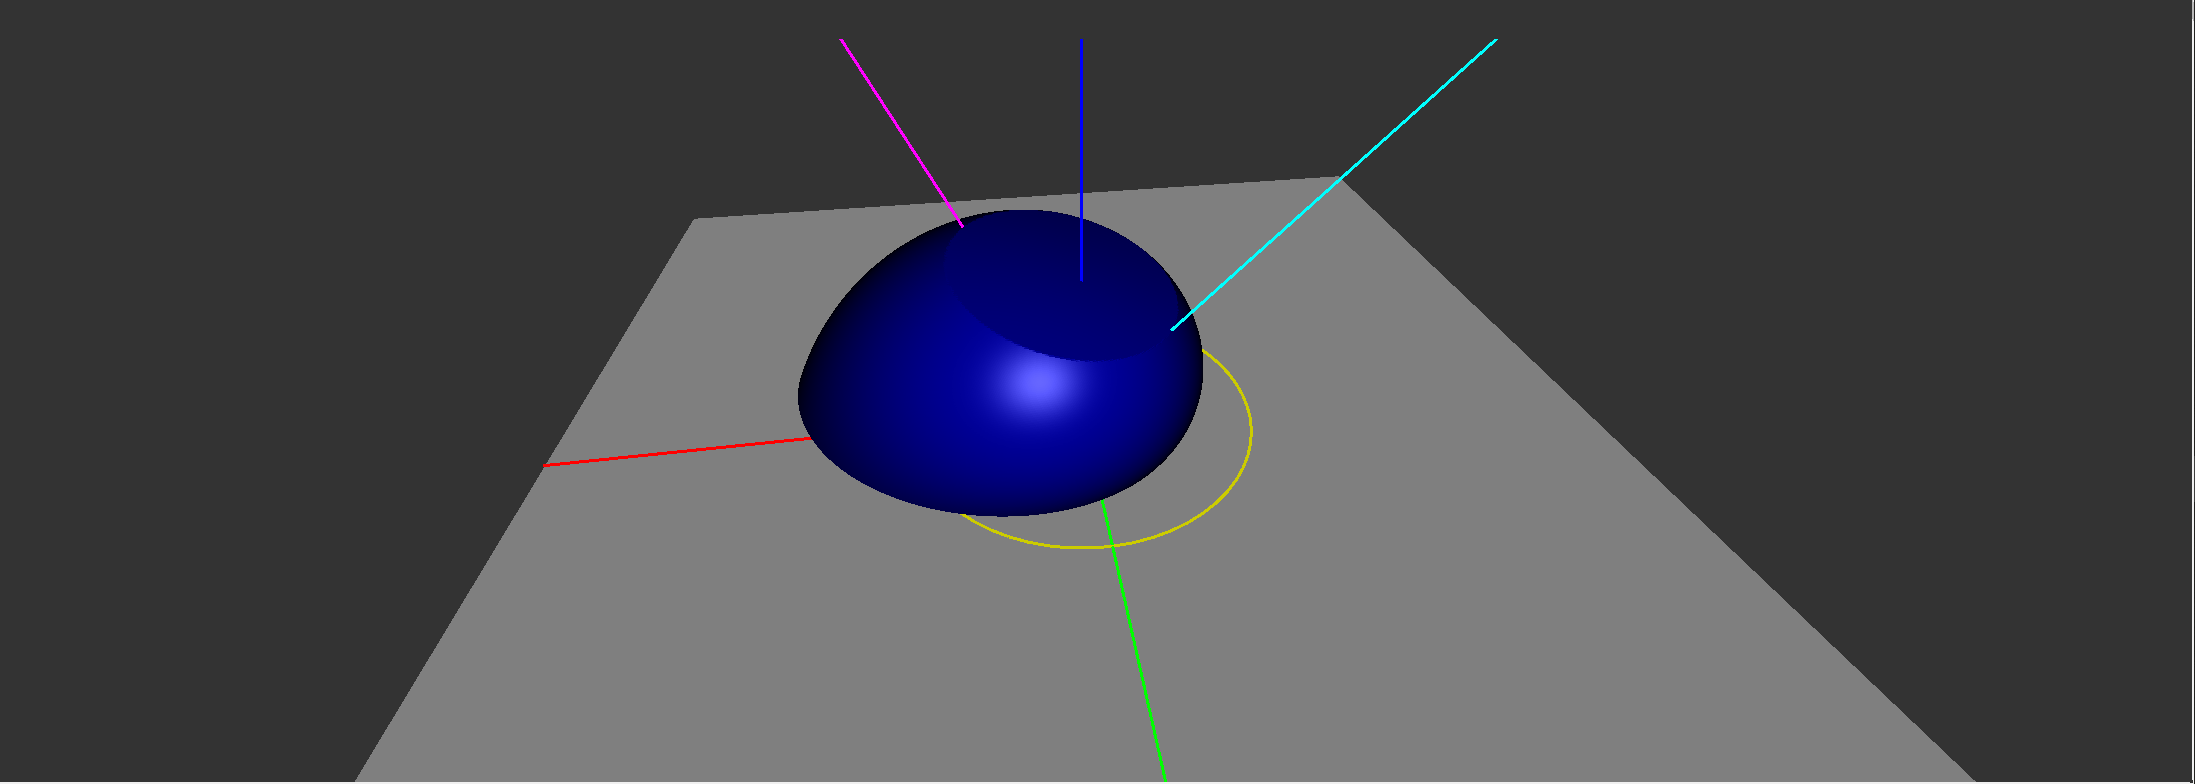
\includegraphics[width=\linewidth]{./Imagens/brdfs/ashikhmin-shirley-alternative-3D-plot}
    % \vspace{0.1px}
    \legend{ \small (a) 3D \textit{plot}}
\endminipage\hfill
\minipage{0.48\textwidth}
  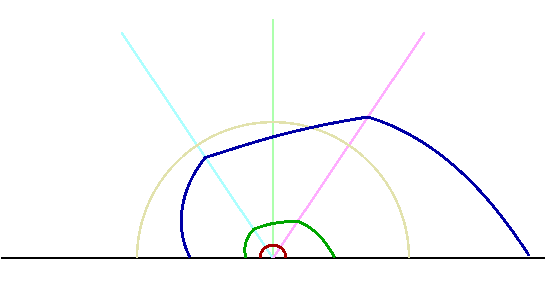
\includegraphics[width=\linewidth]{./Imagens/brdfs/ashikhmin-shirley-alternative-polar-plot.png}
    \legend{ \small (b) \textit{Polar plot}}
\endminipage\hfill
\end{figure}

\begin{figure}[H]
    \caption{\small{Objetos 3D renderizados por este experimento}}\label{fig-ashikhmin-shirley-alternative-eqlang}
\minipage{0.32\textwidth}
  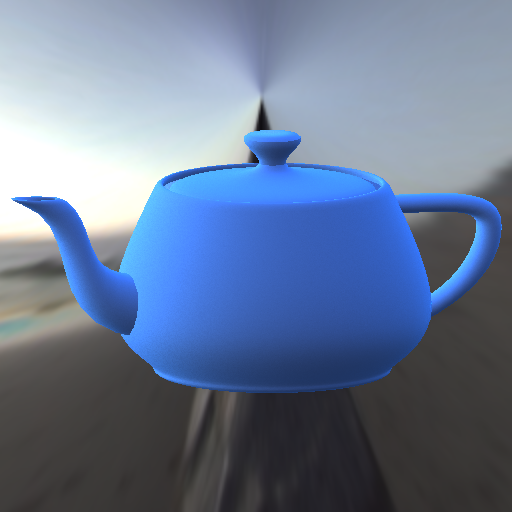
\includegraphics[width=\linewidth]{./Imagens/brdfs/ashikhmin-shirley-alternative-teapot.png}
    \legend{ \small (a) \textit{Teapot}}
\endminipage\hfill
\minipage{0.32\textwidth}
  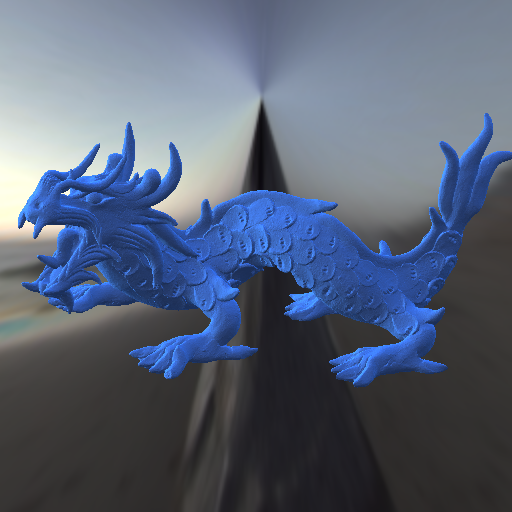
\includegraphics[width=\linewidth]{./Imagens/brdfs/ashikhmin-shirley-alternative-dragon.png}
    \legend{ \small (b) Dragão de Stanford}
\endminipage\hfill
\minipage{0.32\textwidth}%
  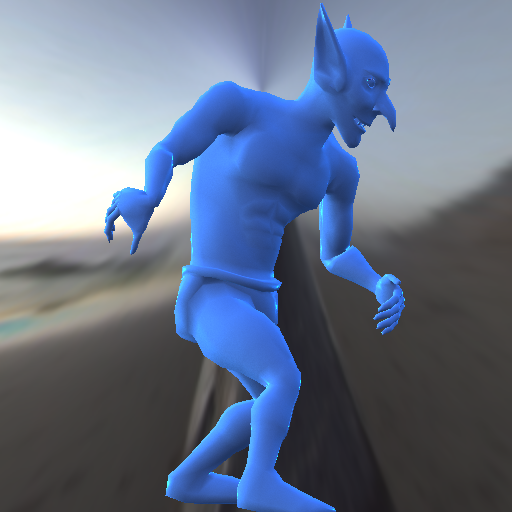
\includegraphics[width=\linewidth]{./Imagens/brdfs/ashikhmin-shirley-alternative-goblin.png}
    \legend{ \small (c) Goblin}
\endminipage
\end{figure}

